In this section we describe the design of a virtual machine scheduling system that manages virtual resources and preparation overhead separately, using scheduling strategies designed to increase accuracy and efficiency. In particular, we will discuss (1) how our scheduling system allocates resources for Best-effort and AR requests, (2) a set of file staging strategies for VM image deployment, and (3) a strategy for reusing VM images on physical nodes.

\section{Best-Effort and AR scheduling}
\label{sec:scheduling}

Our system supports scheduling of best--effort requests and closed advance reservation requests (described in Section~\ref{cha:scenarios}). For best--effort requests, we currently only support serial requests, where the individual VMs in a workspace do not need to run in parallel (this is similar to serial batch jobs). Advance reservations, on the other hand, always request VMs in parallel: all the VMs in an advance reservation will begin at the same time, and a request will be rejected if there are not enough resources for all the VMs at the same time.

A best--effort request includes the following information:

\begin{itemize}
\item[---] Number of VMs in the request. Since the requests will be serial--schedule, each VM is scheduled separately.
\item[---] Resources required by the VMs. These resources are not specified for each VM individually, and a value is provided for all VMs in the same request (e.g., a resource request for 512MB results in each VM requiring that amount of memory). We currently support specifying the number of CPUs and amount of memory required by each VM.
\item[---] Maximum duration of the VMs.
\item[---] VM image required. This information is specified by a URI pointing to the image's location in an image repository node.
\end{itemize}

Best--effort requests are scheduled using a FCFS (First Come First Serve) algorithm. As requests arrive, they are placed on a queue. In turn, the head of the queue is inspected every scheduling quantum, and if there are enough resources to run a single VM at that time, the VM is scheduled for deployment and execution. Since the VMs are serial--scheduled, this process does not involve any backfilling or resource reservation strategies, except in the presence of advance reservations (a case which is explained next).

An advance reservation includes the same information as a best--effort request, plus a specific start time at which all the VMs in the request must start. The end time of the reservation will be computed as \emph{start time + duration}. To schedule advance reservations, our scheduler models physical resources as resource slots (as described in the previous section) where we must fit a given request for an advance reservation. To perform this slot--fitting, we first determine if the request it feasible at the requested start and end times and, if there is a choice of physical nodes, we greedily choose the nodes that would minimize the number of image transfers. This procedure is detailed in Algorithm~\ref{alg:slot}

\begin{algorithm}
\caption{Slot-fitting for advance reservations}
\label{alg:slot}
\begin{algorithmic}
\REQUIRE Request for $n$ VMs, starting at time $t_s$ and ending at time $t_e$, each requiring $r_i$ resources (for all $i$ types of resources: CPU, memory, etc.)
\STATE
\STATE $physNodes[1\ldots m][1\ldots i]:=$ \COMMENT{Array representing $m$ physical nodes. Each physical node has $i$ types of resources}
\STATE
\STATE $candidateNodes:=\emptyset$
\FORALL{$physnode$ in $physNodes$}
\IF{$physnode$ has at least $r_i$ resources from time $t_s$ to $t_e$ (for all $i$ resources)}
\STATE Add $physnode$ to $candidateNodes$
\ENDIF 
\ENDFOR
\STATE
\STATE \COMMENT{$candidateNodes$ now contains all the physical nodes with enough resources to deploy at least one VM}
\STATE
\STATE Sort $candidateNodes$, giving priority to nodes where we will be able to reuse already deployed VM images (see Section~\ref{sec:reuse}), and then to nodes where we can deploy more than one VM.
\STATE
\FORALL{$vm$ in $request$}
\STATE Reserve $r_i$ resources in first available node in $candidateNodes$
\ENDFOR
\STATE
\IF{there are no VMs left to fit}
\STATE \COMMENT{The reservation fits in $candidateNodes$}
\IF{all necessary VM images can be deployed by $t_s$ (see Section~\ref{sec:filestaging})}
\STATE Commit changes to schedule
\ELSE
\STATE Reject
\ENDIF
\ELSE
\STATE Reject
\ENDIF
\end{algorithmic}
\end{algorithm}


\begin{figure}
  \begin{center}
    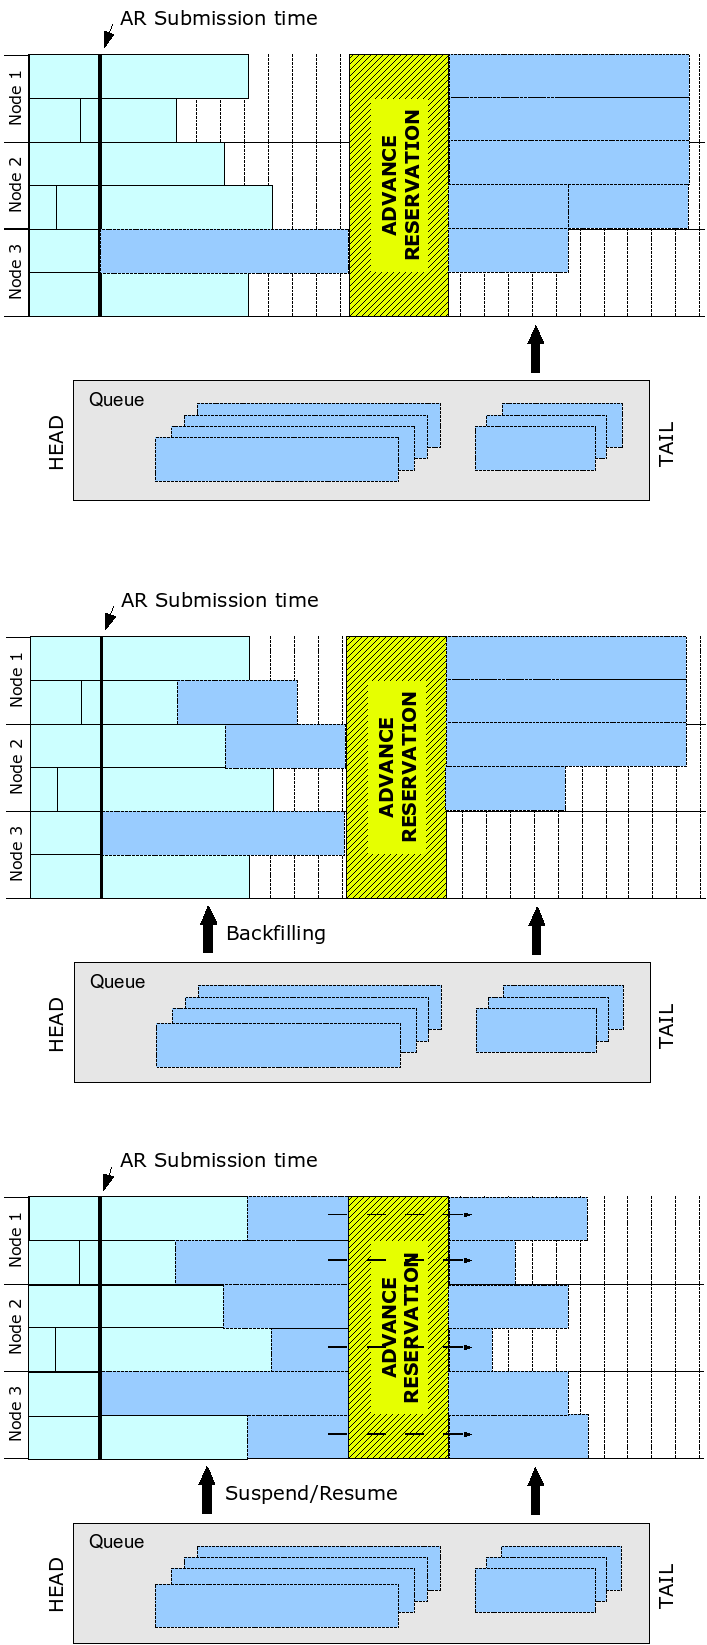
\includegraphics[height=1\textheight]{figures/arbatch.png}
    \caption{Top: Draining nodes before an AR. Middle: Backfilling the time before an AR. Bottom: Suspending before an AR, and resuming after the AR.}
	\label{fig:backfilling}
  \end{center}
\end{figure}


When combining best--effort requests and advance reservations, we can find that the time before an advance reservation is underutilized, as we cannot schedule any best-effort requests that would end after the scheduled start time of the advance reservation (see Figure~\ref{fig:backfilling}, top diagram). This problem is common in parallel job scheduling, where resources can be allocated for a parallel job (requiring several CPUs in parallel), but the resources available before the parallel job might not be able to satisfy the requirements of the next job in the queue. \emph{Backfilling} strategies \cite{10.1109/ICPPW.2002.1039773,feitelson02analyzing,feitelson04parallel} allow lower--priority jobs to run in the time before a parallel job, without affecting the starting times of higher priority jobs (see Figure~\ref{fig:backfilling}, middle diagram).

In a batch scheduler, backfilling strategies differ on how they reserve resources for parallel jobs in the queue. However, our system does not support parallel best--effort requests (the equivalent of parallel jobs in batch schedulers), and we are only interested in backfilling the time before an advance reservation (which cannot be scheduled on a best--effort basis, like a parallel job) with best-effort serial requests. In this case, the task of backfilling becomes much simpler, and is reduced to traversing the queue in search of VMs that can be scheduled before the advance reservation.

However, as shown in Figure~\ref{fig:backfilling}, backfilling can still result in some underutilization. Another alternative is to suspend best--effort requests before an advance reservation, and resume them as soon as the advance reservation ends (see Figure~\ref{fig:backfilling}, bottom diagram). \emph{Suspend/resume} is not a novel strategy, as many existing resource managers, such as Condor and SGE, allow checkpointing of jobs. However, this feature generally requires modifying a job's executable to support checkpointing, although in some cases checkpointing can be achieved by adding support for it to an OS kernel \cite{blcr}. 

As mentioned in Section~\ref{cha:virtualresources}, we currently assume that VMs do not produce any network traffic that would share bandwidth with preparation overhead. In the case of VMs running best--effort requests, we must also assume that these requests do not require any network connections that are essential to completing the request, since it might not be possible to continue these connections after resuming a suspended VM (because of TCP timeouts). This assumption is reasonable in the case of highly parallel applications, where each process is serial--scheduled and there is little or no communication between the individual requests. It should be noted that this restriction does not apply to ARs, since resources are guaranteed to be available during the reservation (i.e., an AR will not be suspended).



\section{File staging strategies}
\label{sec:filestaging}

Jobs submitted to batch schedulers generally assume that the required files are available in the worker nodes (e.g., through an NFS drive) or that the input files will be staged to the worker nodes when the job starts. As discussed in the previous section, this assumption presents problems for deploying time{}-sensitive VWs, as VM images can be large and costly to transfer, and transfer times can consume a significant portion of the time allocated to the user. Thus, even if a resource is made available at a requested time $t$, it may not be ready for use until a significantly later time $t+d$.

These problems can be solved in some cases by providing the scheduler with application--specific information about what data needs to be transferred for each deployment, enabling it to distinguish cases where prestaging the data before the scheduled start time $t$ would be appropriate. In the case of a virtual workspace, the workspace metadata file can serve this purpose. In particular, the relevant information is (1) an image descriptor (currently the location of the image file within an image repository node), (2) the image size, and (3) the number of nodes in the VW.

As described in our virtual resource model, preparation overhead would be managed separately from the virtual resources. Thus, we propose the use of a \emph{scheduled} file transfer strategy: after estimating the amount of preparation overhead, the image transfers are scheduled to complete by time $t$, and the scheduler will reject workspaces where such an image transfer cannot be scheduled (even if all other resources, such as CPU and memory, are available during the requested period of time). In particular, for ARs we schedule image transfers using an Earliest Deadline First (EDF) algorithm \cite{BorjaCite22}. Using EDF allows us to guarantee that image transfers complete by time $t$ (the deadline), while also allowing us to determine which image transfers are infeasible. Since EDF is an aggressive algorithm (image transfers begin as soon as possible, even if the deadline is still far away), we also use a just--in--time variation on EDF, which we term EDF/JIT, where image transfers are still sorted according to their deadlines, but pushed as close as possible to the deadline. Figure~\ref{fig:edf} illustrates these two strategies, and Algorithms~\ref{alg:edf} and~\ref{alg:edfjit} describe the EDF and EDF/JIT algorithms.

\begin{algorithm}
\caption{EDF scheduling of image transfers}
\label{alg:edf}
\begin{algorithmic}
\REQUIRE{An image transfer $imgt$ (containing $duration$ and $deadline$), and an existing image transfer schedule $sched$. Each entry in $sched$ contains $startTime$, $duration$, and $deadline$.}
\STATE
\STATE $nextStart:=sched[0].startTime$
\STATE
\STATE Add $imgt$ to $sched$
\STATE
\STATE Sort $sched$ by $deadline$
\STATE
\STATE \COMMENT{Update start times, and verify that the new schedule is feasible}
\FORALL{$tr$ in $sched$}
\STATE $tr.startTime:=nextStart$
\STATE $endTime:=tr.startTime+tr.duration$
\IF{$endTime > tr.deadline$}
\STATE Reject schedule
\ENDIF
\STATE $nextStart = endTime$
\ENDFOR
\end{algorithmic}
\end{algorithm}

\begin{algorithm}
\caption{EDF/JIT scheduling of image transfers}
\label{alg:edfjit}
\begin{algorithmic}
\REQUIRE{An image transfer $imgt$ (containing $duration$ and $deadline$), and an existing image transfer schedule $sched$. Each entry in $sched$ contains $startTime$, $duration$, and $deadline$.}
\STATE
\STATE Add $imgt$ to $sched$ using EDF algorithm
\STATE
\STATE \COMMENT{Push starting times as close as possible to deadline}
\STATE $nextFeasibleEndTime:=sched[last].startTime + sched[last].duration$
\FORALL{$tr$ in $reverse(sched)$}
\STATE $tr.startTime:=\textrm{earliest}(tr.deadline, nextFeasibleEndTime) - tr.duration$
\STATE $nextFeasibleEndTime:=tr.startTime$
\ENDFOR
\end{algorithmic}
\end{algorithm}

\begin{figure}
  \begin{center}
    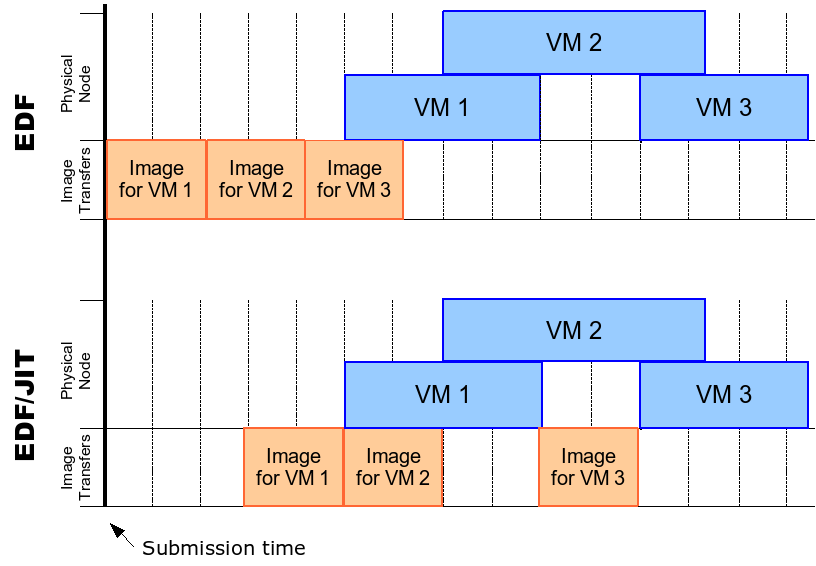
\includegraphics[width=0.8\textwidth]{figures/edf.png}
    \caption{EDF and EDF/JIT file staging strategies}
	\label{fig:edf}
  \end{center}
\end{figure}

Best--effort reservations lack the deadline--sensitive component of AR reservations, so we use a simple FIFO queue to schedule image transfers for these reservations. We currently assume that image transfers for ARs and best--effort reservations are scheduled separately, each having a separate amount of bandwidth they can use exclusively (this separation can be accomplished easily with bandwidth throttling). We leave the development of an algorithm combining the deadline--sensitive aspect of EDF and the best--effort aspect of FIFO, sharing the same bandwidth, for future work.




\section{Reusing VM images}
\label{sec:reuse}

Adequate VM image staging affects \emph{accuracy}, by making sure that all preparation overhead is processed before the virtual workspace's scheduled start time. We also wish to improve \emph{efficiency} by reducing preparation overhead whenever possible. Reducing this overhead allows the scheduler to accept reservations with earlier start times, and benefits best--effort requests by reducing the time spent waiting for image transfer to complete.

We accomplish this goal by reusing VM images already deployed on physical nodes. As described in Section~\ref{sec:vwrepresentation}, factoring deployment--independent configuration information out of the VM image and into a metadata file allows VM images to be reusable. In particular, a VM image can be deployed to a physical machine, and used multiple times by making local copies and binding those copies to potentially different metadata files. This reusability enables us to keep VM image templates on a physical node and use them for several different deployments, thus reducing the number of image transfers.

Our image reuse algorithm requires that each physical node have a certain amount of disk space reserved for an \emph{image pool}. This pool will contain image templates, not bound to any workspace metadata, which can be shared by different deployments. For this sharing to be possible, VMs do not use the images in the pool directly. Instead, if the system supports it, VMs will access images using \emph{copy--on--write} (COW). If COW is not supported, a local copy of the image will be made before the VM starts. Additionally, each image has an expiration time indicating when the image should be removed from the pool. Algorithm~\ref{alg:reuse} describes how the image pool is used when an image has to be transferred to a node.

\begin{algorithm}
\caption{Image reuse}
\label{alg:reuse}
\begin{algorithmic}
\REQUIRE An image $img$ has to be transferred to node $N$, for a VM $v$ starting at $t_\textrm{start}$ and ending at $t_\textrm{end}$. Each node has an image pool $imgpool$. Each entry of $imgpool$ is identified by an image identifier, and contains an expiration time $t_\textrm{expire}$ and a set of VMs $vms$ that will be using that image. 
\STATE
\IF{image pool in node $N$ does \emph{not} have a copy of $img$}
\STATE Transfer image $i$ to node $n$
\STATE Add image to image pool, with $imgId:=i$ and $t_\textrm{expire}=t_\textrm{end}$ \COMMENT{This guarantees that the image will be available for the entire duration of the VM}
\ELSE
\IF{$t_\textrm{start} \leqslant imgpool[img].t_\textrm{expire}$}
\STATE \COMMENT{Image $img$ is guaranteed to be in the image pool at time $t_\textrm{start}$}
\STATE Add $v$ to $imgpool[img].vms$
\STATE $imgpool[img].t_{expire}:=\textrm{max}(imgpool[img].t_\textrm{expire},t_\textrm{end})$
\ELSE
\STATE Transfer and add to pool as described above
\ENDIF
\ENDIF
\end{algorithmic}
\end{algorithm}

When scheduling VWs, the scheduler takes into account the state of the image pools in each node, and attempts to minimize the number of image transfers by allocating, whenever possible, VWs to nodes where the required image is already a part of the image pool. This algorithm also has allows administrators to set a limit on the size of the image pool, making sure that disk usage by VM images will not grow without bounds. The tradeoff, of course, is that some VWs might be rejected since the required VM image is not available in the image pool and cannot be transferred because it would make the image pool too large.



\subsection{Avoiding redundant transfers}

\begin{figure}
  \begin{center}
    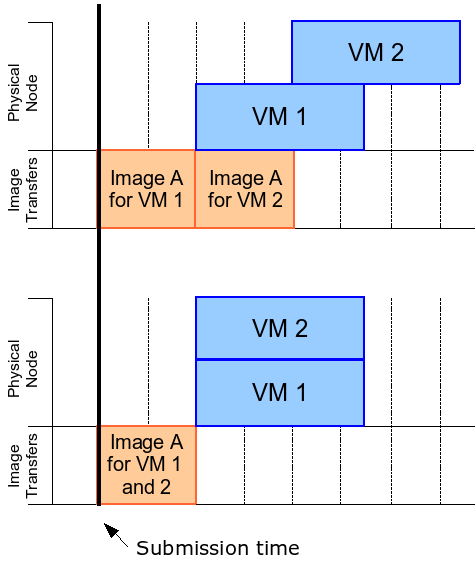
\includegraphics[width=0.6\textwidth]{figures/piggybacking.png}
    \caption{Avoiding redundant transfers}
	\label{fig:piggyback}
  \end{center}
\end{figure}

As an additional optimization to our image reuse algorithm, image transfers are also scheduled in such a way that redundant transfers are avoided. We avoid two types of redundant transfers:

\begin{description}
\item[Transfers for ARs:] Given a VW starting at time $t_\textrm{start}$ and ending at time $t_\textrm{end}$, requiring image $I$, assigned to node $N$. If there is an image transfer of $I$ scheduled to $N$, with deadline less than or equal to $t_\textrm{start}$, then we reuse that transfer. 

For example, assume that a transfer for image $A$ has been scheduled to arrive on node $N1$ at time $t^1_\textrm{start}$. This image will be used by $VW_1$ (ending at $t^1_\textrm{end}$). At some point before $t_\textrm{start}$, a request for $VW_2$ arrives, also requiring image $A$, starting at $t^2_\textrm{start}$ (where $t^2_\textrm{start}>t^1_\textrm{end}$) and ending at time $t^2_\textrm{end}$. The scheduler determines that $VW_2$ should be assigned to node $N1$. Scheduling an additional transfer would be redundant, since there is already a transfer for $A$ scheduled for that node. So, the existing transfer is tagged as carrying an image to be shared by $VM_1$ and $VM_2$. One the transfer is completed, the image's timeout in the pool will be $t^2_\textrm{start}$ (or, more generally, $\textrm{max}(t^1_\textrm{end},t^2_\textrm{end})$)

\item[Transfers for best--effort reservations:] Given a VW requested at time $t_{submit}$ and requiring image $I$, the earliest starting time for that VW will depend on the FIFO transfer queue. More precisely, the scheduler will have to append a transfer to the FIFO transfer queue, ending at time $t_{last-transfer-end}$. If there are enough resources at that time, the earliest starting time for the VW will be $t_{last-transfer-end}$. The scheduler can also check if existing transfers in the FIFO queue could be reused: In particular, the scheduler will look for transfers, each with end time $t_{transfer-end}$ and destination node $N$, such that the image being transferred is image $I$. If there is any transfers such that there are enough resources at time $t_{transfer-end}$ on node $N$, to run the VW, the earliest such transfer is reused.

For example, as shown in Figure~\ref{fig:piggyback} (top), assume that the last image transfer scheduled on the FIFO queue for best--effort reservations carries image $A$ to node $N1$, set to arrive at time $t_\textrm{start}$ to be used by $VM_1$. Also, assume that the time to transfer image A is $t_A$. Now, a request for a new best--effort reservation arrives for $VM_2$, also requiring image $A$. If we scheduled a separate image transfer for $VM_2$, it would start at $t_\textrm{start}+t_A$, despite the availability of resources at $t_\textrm{start}$. By allowing the transfer to piggyback on the previously scheduled transfer, $VM_2$ can start earlier, as show in Figure~\ref{fig:piggyback} (bottom)
\end{description}

In both cases, the scheduler will take into account existing transfers when mapping requests to nodes. Assuming availability of resources in the nodes, it is preferable to schedule a VW to a node with a reusable image transfer than scheduling it to a node where a new image transfer would necessarily have to be scheduled.





